\chapter{Methodology}

\begin{markdown}

This chapter presents the methodology used when developing the PTX.jl
library. Alternative approaches are introduced an discussed with
reasoning for the choises made. Section \ref{sec:meth:ptx} gives a
highlevel overview of the library.

# Julia subset for Kernel definition #

The Julia programming language offers a rich set of abstractions
for increasing programmer productivity. These abstractions incures a
computation overhead at runtime due to indirections and a memory
overhead as the abstractions needs to store more data. This section
describes the subset of Julia used for defining kernels, two separate
methods for implementing the abstractions and a reasoning on the
chosen method.

## The Kernel language ##

In choosing a subset for the kernel language we look at the
application of GPU programs. As they use the SIMT model described in
Section \ref{sec:simt}, arrays fits good to most applications. This
type is chosen along a basic interger.

### Language constructs ###

The basic flow control constructs used in kernel definitions are _if_,
_while_ and _for_\footnote{For loops needs to be short enough to be
  fully unrolled, for all other loops a while must be used}.

## Implementing the Array type ##

There are two obvious methods to implement the types of the kernel
language. On the one hand the types can be realized by implementing
the full Julia abstraction on the GPU. On the other hand one can look
at the implementation or arrays in existing GPU languages as OpenCL C
and CUDA. These two choises both have their benefits and drawbacks
explored in the next sections.

### A full Julia implementation ###

Implementing the Array abstraction from Julia involves including
bounds checking and exception handling giving the programmer a familar
interface to the type. This will ease development for the programmer
could improve programmer productivity when writing kernels. With a
correct implementation the Julia semantics would be continued on the
GPU. The implementation is complicated by the fact that extra
datatypes must be defined on the GPU and new copy functions must be
added. The method does not trivialy imply a efficient implementation
as the will be overhead both on element access and data movement.

### A low level implementation ###

Implementing the Array type as a unboxed array implies getting rid of
size information and leaving the task of bounds checking to the
programmer. This approach is the simpler of the two as the
implementation of a unboxed array is quite simple. On the upside this
will enable integration with existing tools like the CUDA.jl or
OpenCL.jl libraries for transfering data to and from the GPU as these
expect the data to be unboxed arrays on the GPU. This method produces
efficient code trivially as there is no overhead compared to existing
low level solutions.

### Choosing the Low level implementation ###

The Low Level implementation is chosen as it is simpler to implement
and will provide efficient code without resolving to custom
optimizations. This lets the makes the implementation feasable in the
time window and lets the focus be on a fully working system. 

# External library vs. component of the compiler #

The obvious placement of a software component that generates code for
a new platform for a programming language, is in the code generator
module of the _compiler_/_interpreter_. This enables the module to
access the AST of the language in an in-memory format. This also
implies that the source code of the compiler has to be changed for
adoption of the component. An alternative approach is the implement
the component as a separat _library_. In order to do so we need to get
the AST in some other way. This enables the new target to be used
without changing the compiler. The first approach is according to the
Julia mailing list in the making. The first draft is so deeply
intertwined with the current code generator that the authors decided
not to publish their work. A refactoring of this version is
underway. In light of this and the fact that the simplistic design
taken in PTX.jl enables a library approach, this was chosen. This
enables easily adoption and rapid prototyping and improvments to the
library. Even though PTX.jl is a separat library, the LLVM
optimization passes developed for the library should be easy to
integrate into a future compiler with a PTX code generator.

# The PTX.jl library #
\label{sec:meth:ptx}
  
The PTX.jl library generates NVIDIA PTX code from a Kernel defined in
the Julia programming language. The library is developed as a Julia
module and can easily be included in a Julia program. It interopts
with existing 

## Main idea ##

The main idea for generating the GPU code is to substitute Julia
arrays with unboxed arrays. And provide a low level implementation of
the methods operating on the arrays for C like pointers. When
inlineing for the functions operating on the array types are disabled,
the LLVM IR generated resembles a highlevel description of the kernel
that can be translated into a low level implementation on
pointers. This fact is exploted and low level implementation of the
highlevel Julia functions _getindex_ and _setindex_ are linked with
the code. In addition to support the OpenCL programming model, builtin
functionality like _get_global_id_ is also linked.

\begin{figure}[H]
  \centering
  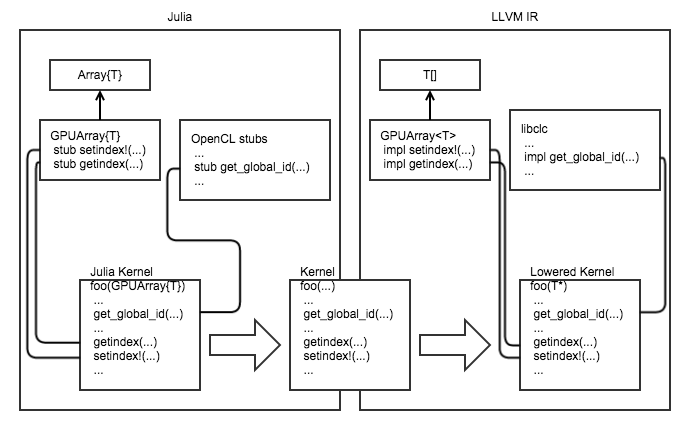
\includegraphics[width=1\textwidth]{body/figures/lowering_schematic.png}
  \caption{Schematic for lowering kernel functions}
  \label{fig:lowering}
\end{figure}

In Figure \ref{fig:lowering} the kernel is linked to the Julia stubs
for getindex, setindex and get_global_id on the left side. The
parameter type for the function is a Julia boxed array. The function
parameter is replaced by the unboxed version of the array and the type
is propagated through the function. As the GPUArray only
implements\footnote{This is using termonology from OOP. Julia does not
  use this termonology, but the language features does enable OOP. In
  Julia termonology the only functions that have methods that accept
  GPUArray as parameters are setindex and getindex.} the functions
setindex and getindex, we are guarantied that the array is not
referenced in other contexts than through these accessor functions.
Linking these two methods with implementations for unboxed arrays
concludes the lowering of the functions. The remaining task is to
provide implementations for the OpenCL builtin functions. This is done
by linking to an open source library called libclc.

  
\end{markdown}
